\documentclass[a4paper]{article}

\usepackage[a4paper, left=3cm, right=2cm, top=2cm, bottom=2cm]{geometry}

% Times New Roman
\usepackage{fontspec}
\setmainfont{Times New Roman}

% Single line spacing + 3pt paragraph spacing
\usepackage{setspace}
\singlespacing
\setlength{\parskip}{3pt}
\setlength{\parindent}{1cm}

% Font size 13pt (all relative sizes scale correctly)
\usepackage[fontsize=13pt]{fontsize}

\usepackage{cite}
\usepackage{amsmath}
\usepackage{graphicx}
\usepackage{booktabs}
\usepackage{array}
\usepackage{url}
\usepackage{listings}
\usepackage{ragged2e}
\lstdefinestyle{mystyle}{
    backgroundcolor=\color{gray!10},   
    commentstyle=\color{green!60!black},
    keywordstyle=\color{blue},
    numberstyle=\normalsize\color{gray},
    stringstyle=\color{purple},
    basicstyle=\ttfamily\normalsize,
    breaklines=true,                   % Automatically wrap long lines
    captionpos=b,                      % Caption at the bottom
    keepspaces=true,                   % Keeps spaces for indentation
    numbers=left,                      % Line numbers on the left
    numbersep=5pt,                     
    showspaces=false,                  
    showstringspaces=false,
    showtabs=false,                    
    tabsize=2,
    columns=fullflexible
}
\lstset{style=mystyle}
\usepackage{indentfirst}
\usepackage{float}
\usepackage{tikz}
\usetikzlibrary{
	arrows.meta,
	calc,
	shapes,
	shapes.misc,
	shapes.arrows,
	chains,
	matrix,
	positioning,
	scopes,
	decorations.pathmorphing,
	shadows
}

\graphicspath{{./}{paper/}{paper/figures/}}

% =====================================================================
% Formatting to match the Vietnamese science-fair report layout
% (cover page, table of contents, list of figures, list of tables)
% =====================================================================
\usepackage{titlesec}
\usepackage{tocloft}
\usepackage[labelsep=period]{caption}

% Section numbering: PART I, PART II, ... and subsections I.1, I.2, ...
\renewcommand{\thesection}{\Roman{section}}
\renewcommand{\thesubsection}{\thesection.\arabic{subsection}}
\titleformat{\section}{\normalfont\Large\bfseries}{PART \thesection:}{0.5em}{}
\titleformat{\subsection}{\normalfont\normalsize\bfseries}{\thesubsection.}{0.5em}{}

% Caption names
\renewcommand{\figurename}{Figure}
\renewcommand{\tablename}{Table}

% Headings of the front-matter lists
\renewcommand{\contentsname}{TABLE OF CONTENTS}
\renewcommand{\listfigurename}{LIST OF FIGURES}
\renewcommand{\listtablename}{LIST OF TABLES}

% Centered, bold list titles
\renewcommand{\cfttoctitlefont}{\hfill\normalsize\bfseries}
\renewcommand{\cftaftertoctitle}{\hfill\null}
\renewcommand{\cftloftitlefont}{\hfill\normalsize\bfseries}
\renewcommand{\cftafterloftitle}{\hfill\null}
\renewcommand{\cftlottitlefont}{\hfill\normalsize\bfseries}
\renewcommand{\cftafterlottitle}{\hfill\null}
\setlength{\cftbeforetoctitleskip}{0pt}
\setlength{\cftaftertoctitleskip}{6pt}
\setlength{\cftbeforeloftitleskip}{18pt}
\setlength{\cftafterloftitleskip}{6pt}
\setlength{\cftbeforelottitleskip}{18pt}
\setlength{\cftafterlottitleskip}{6pt}

% TOC entries: "PART I: ...", bold, dotted leaders
\renewcommand{\cftsecfont}{\bfseries}
\renewcommand{\cftsecpagefont}{\bfseries}
\renewcommand{\cftsecpresnum}{PART~}
\renewcommand{\cftsecaftersnum}{:}
\renewcommand{\cftsecleader}{\bfseries\cftdotfill{\cftdotsep}}
\setlength{\cftsecnumwidth}{6.5em}
\setlength{\cftbeforesecskip}{4pt}

\renewcommand{\cftsubsecfont}{\bfseries}
\renewcommand{\cftsubsecpagefont}{\normalfont}
\renewcommand{\cftsubsecaftersnum}{.}
\setlength{\cftsubsecindent}{1em}
\setlength{\cftsubsecnumwidth}{5.5em}

% List of figures: "Figure 1. ..."
\renewcommand{\cftfigpresnum}{Figure~}
\renewcommand{\cftfigaftersnum}{.}
\setlength{\cftfigindent}{0pt}
\setlength{\cftfignumwidth}{4.8em}

% List of tables: "Table 1. ..."
\renewcommand{\cfttabpresnum}{Table~}
\renewcommand{\cfttabaftersnum}{.}
\setlength{\cfttabindent}{0pt}
\setlength{\cfttabnumwidth}{4.8em}

\begin{document}
	
	% ================= PAGE 1: COVER PAGE =================
	\thispagestyle{plain}
	\begin{center}
		\bfseries
		SCHOOL-LEVEL SCIENCE AND ENGINEERING FAIR FOR SECONDARY SCHOOL STUDENTS, SCHOOL YEAR 2026 -- 2027
	\end{center}
	
	\vspace{5cm}
	
	\begin{center}
		\bfseries
		REPORT ON THE RESEARCH'S FINDINGS
	\end{center}
	
	\vspace{3cm}
	
	\begin{center}
		{\Large\bfseries\itshape Project title:}\\[10pt]
		{\Large\bfseries
		\MakeUppercase{MemoLang: Research and Development of a Buffer-Release Mechanism for AI Development}\par}
	\end{center}
	
	\vspace{3cm}
	
	\noindent\textbf{\textit{Category:} Systems Software}
	
	\vspace{6pt}
	
	\vfill
	
	\begin{center}
		\textbf{\textit{Hanoi, September 2026}}
	\end{center}
	
	\newpage
	
	% ================= PAGES 2–3: TOC + LISTS =================
	\tableofcontents
	
	\listoffigures
	\listoftables
	
	% ----- LIST OF ABBREVIATIONS -----
    \vspace{10cm}
	\vspace{18pt}
	\begin{center}
		\textbf{LIST OF ABBREVIATIONS}
	\end{center}
	\vspace{-6pt}
	\begin{center}
		\renewcommand{\arraystretch}{1.15}
		\begin{tabular}{>{\bfseries}l >{\raggedright\arraybackslash}p{5.8cm} >{\raggedright\arraybackslash}p{5.8cm}}
			\toprule
			\textbf{Abbreviation} & \textbf{Full name} & \textbf{Description} \\
			\midrule
			AI      & Artificial Intelligence & Computer systems that perform tasks normally requiring human intelligence \\
			AOT     & Ahead-Of-Time (compilation) & Compiling code to machine code before the program runs \\
			AST     & Abstract Syntax Tree & Tree representation of the structure of source code \\
			cuBLAS  & CUDA Basic Linear Algebra Subprograms & NVIDIA's GPU-accelerated linear algebra library \\
			CUDA    & Compute Unified Device Architecture & NVIDIA's parallel computing platform for GPUs \\
			CUTLASS & CUDA Templates for Linear Algebra Subroutines & NVIDIA's open-source C++ template library for GEMM kernels \\
			DRAM    & Dynamic Random-Access Memory & Main memory that must be periodically refreshed \\
			FFI     & Foreign Function Interface & Mechanism for calling functions written in another language \\
			GEMM    & General Matrix Multiplication & Standard routine for multiplying two matrices \\
			GPU     & Graphics Processing Unit & Processor specialized for highly parallel computation \\
			IR      & Intermediate Representation & Code form used inside a compiler between source and machine code \\
			JIT     & Just-In-Time (compilation) & Compiling code to machine code while the program runs \\
			LLVM    & LLVM Compiler Infrastructure (originally ``Low Level Virtual Machine'') & Toolkit for building compilers and code generators \\
			MatMul  & Matrix Multiplication & Multiplication of two matrices \\
			REPL    & Read--Eval--Print Loop & Interactive shell that evaluates input line by line \\
			\bottomrule
		\end{tabular}
	\end{center}
	
	
	\newpage
	
	% ================= MAIN CONTENT =================
	\section{Project Overview}
	\label{sec:overview}
	
	\subsection{Rationale}
	
	The recent development of AI has led to an explosion of machine learning algorithms and deep learning models. As a result, the demand for computing power to train on enormous datasets has also increased.
	
	Currently, one of the most widely used operations in machine learning algorithms is GEMM. During training, each matrix multiplication produces another matrix, and this new matrix is in turn fed into further matrix multiplications. To handle many different operations, tasks and processes, machine learning models need to perform millions of matrix computations. Because these matrix computations are far more time-intensive than ordinary computations, subsequent computations gradually pile up in buffer memory and intermediate steps until memory-management programs or the system's rules free the memory.
	
	Repeating this process becomes a major problem for machine learning models operating under very large workloads, with serious consequences for the performance and latency of the model on the device and hardware resources it uses.
	
	Therefore, this software aims to optimize memory management around GEMM operations, ensuring that buffers, buffered data and pointers are freed as early as possible and reducing the overhead caused by buffer accumulation.
	
	This project was inspired by research into destructive-read memory systems, the Sere programming language~\cite{sere}, the Clean programming language~\cite{clean}, and optimized GPU matrix-multiplication libraries.
	
	\subsection{Research Questions}
	
	Inherent overheads, as well as the risk of overestimating memory overhead or the practicality of memory optimization, must be considered. Therefore, the project investigates the following hypotheses:
	
	\begin{itemize}
		\item Destructive-read semantics can reduce peak memory usage for workloads containing short-lived intermediate matrices.
		\item Destructive reads can reduce the number or cost of temporary-buffer allocations when consumed buffers can safely be reused.
		\item For workloads in which memory management represents a significant portion of total execution time, buffer reuse may improve end-to-end performance.
	\end{itemize}
	
	\subsection{Research Objectives}
	
	The goal of the language is to determine whether language-level destructive-read semantics can provide measurable memory-management benefits for matrix-oriented GPU programs while retaining the performance of optimized matrix multiplication kernels.
	
	The project will be implemented and evaluated through the following goals:
	
	\begin{enumerate}
		\item Define the language's core Python-like syntax and destructive-read semantics.
		\item Implement a lexer, parser, AST, and LLVM-based code-generation pipeline.
		\item Generate LLVM IR for arithmetic and matrix operations.
		\item Integrate optimized GPU matrix multiplication through cuBLAS.
		\item Implement explicit ownership and consumption tracking for matrix operands.
		\item Determine when consumed matrix buffers can safely be reused.
		\item Verify generated results against an independent numerical reference.
		\item Measure peak GPU memory usage and temporary-buffer allocation behavior.
		\item Measure both GPU kernel execution time and end-to-end program runtime.
		\item Compare destructive-read execution against an equivalent non-destructive implementation.
		\item Compare the language against optimized GPU-library baselines where appropriate.
		\item Preserve benchmark logs, correctness results, compiler output, and build artifacts to make the experimental results reproducible.
	\end{enumerate}
	
	\subsection{Novelty}
	
	The novelty of the project lies in directly linking the precompiled \emph{cuBLAS runtime library}~\cite{cublas} for a specific application, evaluated with a specific methodology, under an enforcement model resembling a \emph{strictly linear type system}. Other languages have pursued related consumption-tracking semantics: Rust's ownership system~\cite{rust} enforces a comparable use-once discipline through its affine type system, and Futhark~\cite{futhark} is a purely functional array language that uses uniqueness types to support safe in-place updates. Futhark, however, generates its own GPU kernels from source rather than integrating with external, independently maintained high-performance libraries such as cuBLAS, a limitation that has been noted as one of the practical hurdles of the language. The language instead separates compile-time consumption analysis from kernel execution.

	In addition to cuBLAS, a separate GEMM kernel will be integrated directly using \emph{CUTLASS}~\cite{cutlass}, NVIDIA's open-source template library for GEMM. Because CUTLASS kernels are instantiated at compile time rather than called as opaque precompiled routines, this path gives the runtime direct control over operand and workspace buffers, allowing consumed buffers to be released or reused at a finer granularity than the cuBLAS interface permits. Like cuBLAS, CUTLASS is an external, independently maintained library, so the language still avoids generating its own kernels from source.
	
	\section{Background}
	
	Matrix multiplication can be written as
	
	\begin{equation}
		C_{i,j} = \sum_{k=0}^{N-1} A_{i,k}B_{k,j}
	\end{equation}
	
	Each value in the output matrix $C$ is produced by multiplying one row of $A$ with one column of $B$ and summing the products. Efficient implementations must manage data movement, memory reuse and the lifetime of operand buffers.
	
	\begin{equation}
		T_1 = A B,\qquad
		T_2 = T_1 C,\qquad
		T_3 = T_2 D,
	\end{equation}
	
	In practice, numerous intermediate buffers are live at the same time. Ideally, the storage of these buffers should be released and reused as soon as their respective operations complete or their lifetime ends.
	
	
	Destructive-read is a memory read operation that inherently erases the value it reads: data is destroyed at the same time it is accessed. If a value must be preserved, a write-back operation must immediately restore it, or an external buffer/cache must hold a copy.
	
	Related work on linear type systems takes a similar approach at the language level, requiring that a variable be used exactly once.
	
	Destructive-read has, historically, been more common in hardware and circuit design than in software. Dybdahl et al.~\cite{DybdahlKGN06} studied destructive-read behavior in embedded DRAM and found that removing the write-back buffer and instead relying on the cache by reading data into the cache without immediately restoring it to DRAM, and writing it back only when the cache line is replaced, offered measurable power and performance benefits. 
	
	While that result is specific to a hardware memory system, it motivates the broader question this project investigates: whether a comparable consume-on-read discipline, applied at the software/interpreter level for GEMM-heavy workloads, can yield similar results.
	
	
	\subsection{Destructive-Read Semantics}
	
	A destructive read treats a value as consumed when an operation has exclusive use of that value. After consumption, the original value is no longer available to subsequent operations unless the programmer explicitly creates a copy or otherwise preserves it.
	
	For matrix operations, this provides an opportunity for storage reuse. For example,
	
	\begin{align*}
		C &= A \mathbin{@} B\\
		D &= C \mathbin{@} W
	\end{align*}
	
	\noindent where $\mathbin{@}$ denotes matrix multiplication. This may permit the storage associated with $A$ or $C$ to become eligible for reuse once the compiler establishes that the corresponding value has no remaining consumers.
	
	The purpose of this mechanism is not to alter the mathematical computation performed by matrix multiplication. Instead, it changes the lifetime of buffers associated with the computation. If a buffer can be reused without copying its contents, the implementation may reduce peak memory consumption and allocation activity.
	
	This optimization is inherently workload-dependent. A matrix with multiple future consumers cannot safely be destroyed after its first use. In such cases, the implementation may require a copy, borrow, or other mechanism to preserve the value. Consequently, destructive-read semantics can introduce a tradeoff between memory efficiency and the flexibility to reuse values.
	
	The language therefore treats destructive reads as an explicit ownership mechanism rather than assuming that consuming every operand will necessarily improve performance.
	
	\section{Design and Methodology}
	
	\subsection{Syntax Design}
	
	We adopted a Python-like syntax convention for the language:
	\begin{itemize}
		\item Comments using the hash sign (\#).
		\item Primitive types: Integer, Float, Boolean and String.
		\item Variable declarations.
		\item Functions defined with `def'.
		\item \texttt{extern} for runtime/FFI (cross-language) linkage.
		\item Operator precedence.
		\item Control flow.
	\end{itemize}
	However, for implementation practicality and other design reasons, we made the following adjustments to the core Python syntax:
	\begin{itemize}
		\item A built-in \texttt{copy()} that copies a matrix, for keeping a matrix that an operation would otherwise consume.
		\item Braces instead of indentation for function scope.
	\end{itemize}
	
	\subsection{Pipeline}
	The complete pipeline of the language, from source text to GPU execution, is shown in Figure~\ref{fig:pipeline}. Code generation is built on the LLVM compiler infrastructure~\cite{llvm}.
	\begin{figure}[H]
		\centering
		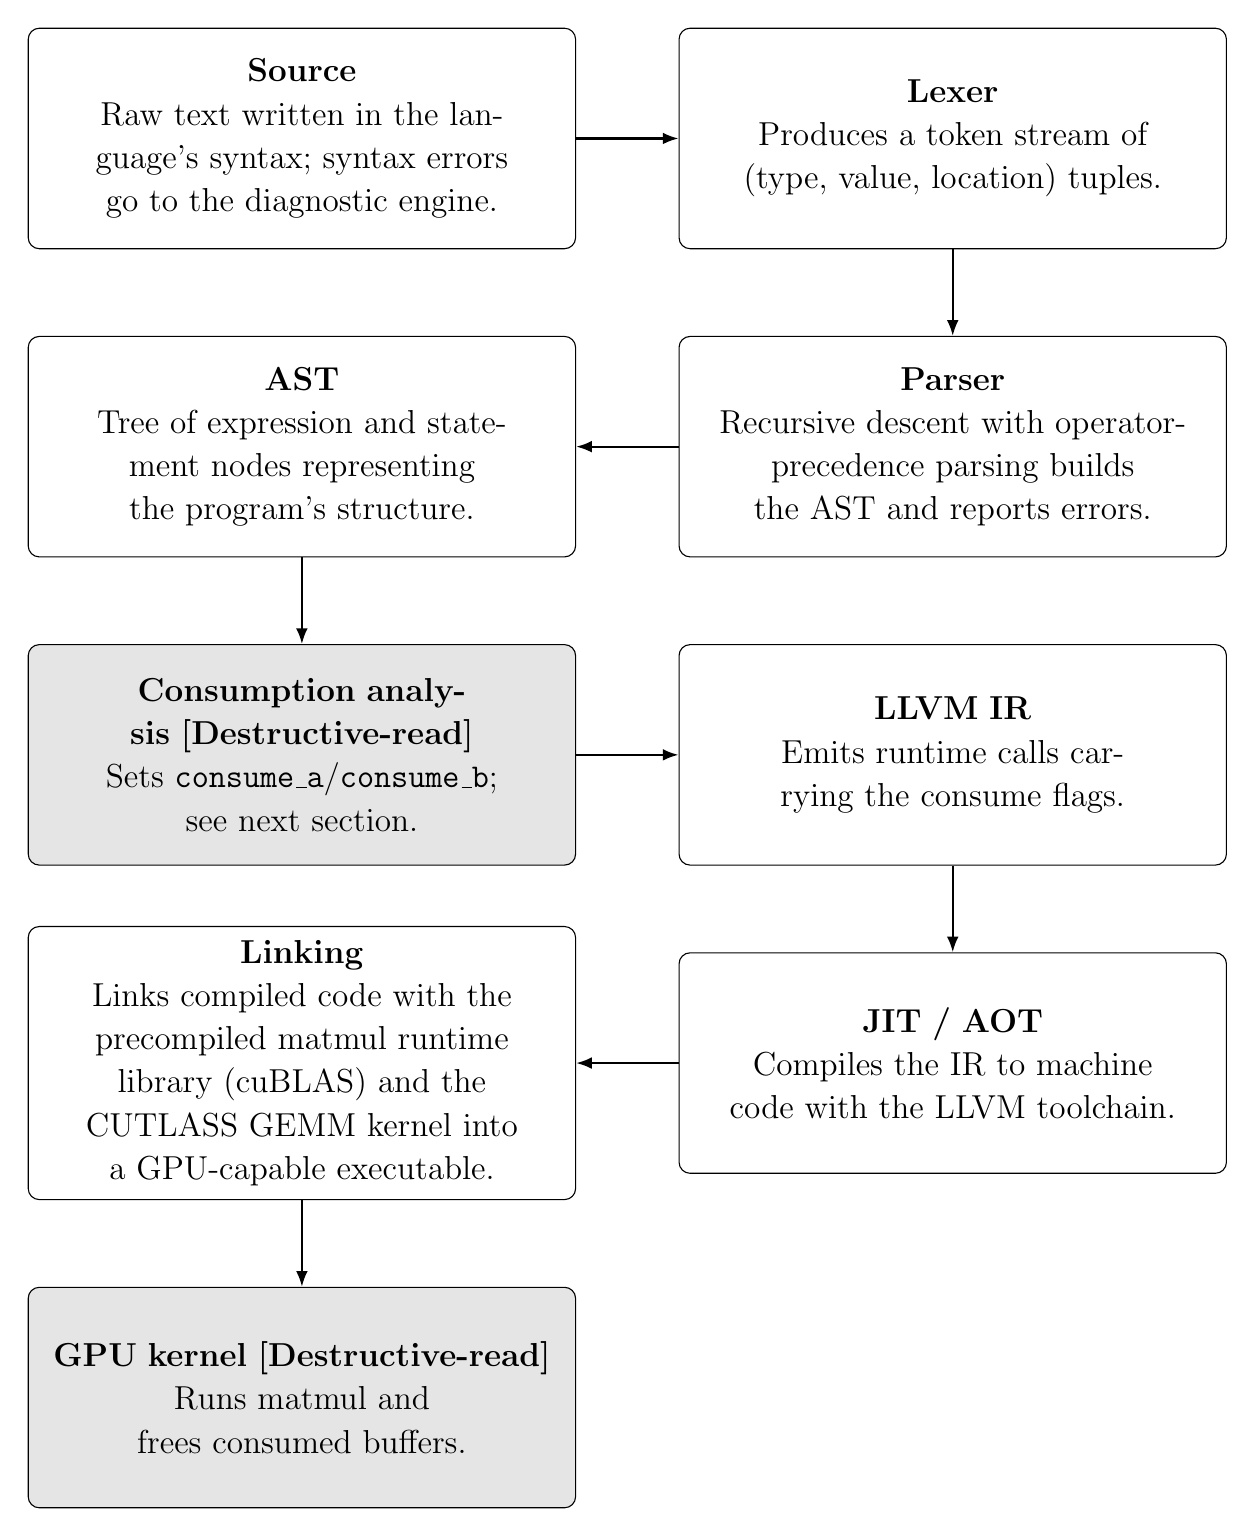
\begin{tikzpicture}[
			node distance=1.1cm and 1.3cm,
			box/.style={
				rectangle, draw, rounded corners,
				text width=6.6cm,
				minimum height=2.8cm,
				inner sep=5pt,
				align=center,
				font=\normalsize
			},
			special/.style={box, fill=gray!20},
			arr/.style={-{Latex[length=2mm]}, thick}
			]
			
			\node[box] (src) {\textbf{Source}\\
				Raw text written in the language's syntax; syntax errors go to the diagnostic engine.};
			\node[box, right=of src] (lex) {\textbf{Lexer}\\
				Produces a token stream of (type, value, location) tuples.};
			\node[box, below=of lex] (par) {\textbf{Parser}\\
				Recursive descent with operator-precedence parsing builds the AST and reports errors.};
			\node[box, left=of par] (ast) {\textbf{AST}\\
				Tree of expression and statement nodes representing the program's structure.};
			\node[special, below=of ast] (con) {\textbf{Consumption analysis [Destructive-read]}\\
				Sets \texttt{consume\_a}/\texttt{consume\_b}; see next section.};
			\node[box, right=of con] (ir) {\textbf{LLVM IR}\\
				Emits runtime calls carrying the consume flags.};
			\node[box, below=of ir] (jit) {\textbf{JIT / AOT}\\
				Compiles the IR to machine code with the LLVM toolchain.};
			\node[box, left=of jit] (link) {\textbf{Linking}\\
				Links compiled code with the precompiled matmul runtime library (cuBLAS) and the CUTLASS GEMM kernel into a GPU-capable executable.};
			\node[special, below=of link] (gpu) {\textbf{GPU kernel [Destructive-read]}\\
				Runs matmul and frees consumed buffers.};
			
			\draw[arr] (src) -- (lex);
			\draw[arr] (lex) -- (par);
			\draw[arr] (par) -- (ast);
			\draw[arr] (ast) -- (con);
			\draw[arr] (con) -- (ir);
			\draw[arr] (ir) -- (jit);
			\draw[arr] (jit) -- (link);
			\draw[arr] (link) -- (gpu);
		\end{tikzpicture}
		\caption{Compilation pipeline of the language. Shaded boxes denote where destructive-read semantics are relevant.}
		\label{fig:pipeline}
	\end{figure}
	
	\subsection{The Free-on-Consume Scheme and cuBLAS runtime}
	The scheme referenced in~\cite{DybdahlKGN06} will be used with a modified design philosophy to work at a software level; the design choices are summarised in Table~\ref{tab:scheme_implementation}.

	For cuBLAS pre-compile linking:
	\begin{itemize}
		\item cuBLAS should be dynamically linked.
		\item Driver should link and ship with compiled binaries from cuBLAS.
		\item For convenience, distributed as a packaged file.
	\end{itemize}

	For the separate CUTLASS GEMM kernel:
	\begin{itemize}
		\item The kernel is built from CUTLASS templates and compiled together with the runtime, rather than linked as a prebuilt binary.
		\item The runtime passes consume flags to the kernel wrapper so that consumed operands can be freed or reused as the output or workspace buffer.
		\item cuBLAS and the CUTLASS kernel are benchmarked against each other on the same workloads.
	\end{itemize}
	
	\begin{table}[H]
  \centering
  \caption{Scheme implementation choices in the design.}
  \label{tab:scheme_implementation}
  \begin{tabular}{@{}>{\RaggedRight}p{0.48\linewidth} >{\RaggedRight}p{0.48\linewidth}@{}}
    \toprule
    \textbf{Scheme} & \textbf{Implementation} \\
    \midrule
    Data is first read from DRAM into the cache. 
      & No difference. \\ \addlinespace
    
    Data is written back to DRAM when the cache line is replaced, regardless of whether data was modified. 
      & Operands are freed unconditionally under the assumption that the cache is always modified. \\ \addlinespace
    
    Reuses existing cache architecture. 
      & Uses scope-exit allocation for cache management. \\ \addlinespace
    
    Hides write-back latency using multi-bank overlap (bank interleaving). 
      & Hides memory free overhead behind GPU kernel launches. \\
    \bottomrule
  \end{tabular}
\end{table}

	
	\section{Process, Creation and Testing}
	
	\subsection{Process}
	
	The compiler is written in C++20. Each stage is first designed, then coded, then debugged independently to look for errors, and the stages are then assembled modularly. Every stage reports errors through one diagnostic engine, so all messages share one format and point at the exact source text. The main source folders are listed in Table~\ref{tab:modules}. Until code generation exists, checked programs are run by an interpreter on a CPU matrix runtime, which is also what the measurements in Section~\ref{sec:evidence} use.

	\begin{table}[h]
		\centering
		\caption{Main Source Folders}
		\label{tab:modules}
		\begin{tabular}{@{}>{\RaggedRight}p{0.36\linewidth} >{\RaggedRight}p{0.58\linewidth}@{}}
			\toprule
			Folder & Purpose \\
			\midrule
			\texttt{Include/Source/} & Reads source files; maps positions to line and column \\
			\texttt{Include/Diag/} & Diagnostic engine (error messages) \\
			\texttt{Include/Lex/} & Lexer: source text to tokens \\
			\texttt{Include/Parser/} & Parser: tokens to the abstract syntax tree (AST) \\
			\texttt{Include/AST/} & AST node definitions and printer \\
			\texttt{Include/Types/} & Semantic types, including matrices \\
			\texttt{Include/Semantics/} & Semantic analysis: names and types \\
			\texttt{Include/Analysis/} & Consumption (destructive-read) analysis \\
			\texttt{Include/Interp/} & Interpreter: runs checked programs \\
			\texttt{Include/Runtime/} & CPU matrix runtime with memory accounting \\
			\texttt{Include/IR/} & LLVM IR generation (interface only) \\
			\texttt{Include/Driver/}, \texttt{main.cpp} & Command-line program \\
			\texttt{tests/}, \texttt{benchmarks/} & Automated tests and benchmark programs \\
			\bottomrule
		\end{tabular}
	\end{table}
	
	\subsection{Testing}

	The project has 27 automated tests (Table~\ref{tab:verification}). They run on every change, on Windows (MSVC) and Linux (GCC), in Debug and Release builds. All 27 pass.

	\begin{table}[h]
		\centering
		\caption{Correctness Test Results}
		\label{tab:verification}
		\begin{tabular}{@{}>{\RaggedRight}p{0.70\linewidth} >{\RaggedRight}p{0.24\linewidth}@{}}
			\toprule
			Test Case & Result \\
			\midrule
			Lexer and parser output compared line by line with expected output (8 files) & Pass \\
			Syntax errors: 36 deliberate mistakes, each reported exactly once & Pass \\
			Semantic errors: 38 deliberate mistakes (names, types, calls) & Pass \\
			Destructive-read re-use detection: 9 uses of a consumed matrix, found at compile time, including after a branch and in a later loop iteration & Pass \\
			Valid programs accepted with no errors (2 files) & Pass \\
			Matrix multiplication against a reference: identity $\times$ $M = M$ for square and non-square matrices, and identical results across four implementations (Section~\ref{sec:evidence}) & Pass \\
			Arithmetic and control flow when running programs (20 checks) & Pass \\
			Shape mismatch detected while running & Pass \\
			No memory leaks: every allocated matrix freed, in both modes & Pass \\
			Stress tests: 36 extreme inputs (100\,000-deep nesting, 1~MB lines, 10\,000-term chains) & Pass \\
			Fuzzing: 9\,000 random inputs, no crash or hang & Pass \\
			\bottomrule
		\end{tabular}
	\end{table}

	\begin{itemize}
		\item Matrix multiplication against a reference: every benchmark computes the same result in all four implementations, and multiplying by the identity matrix returns the original matrix, including for non-square matrices.
		\item Destructive-read re-use detection: the compiler rejects any use of a matrix after it has been consumed, before the program runs; a note shows where the matrix was consumed.
		\item Edge cases: empty files, 1~MB inputs, very deep nesting, very long chains and random input are all handled without a crash.
	\end{itemize}
	
	
	\subsection{Benchmarks}
	
	The benchmark evaluation is designed to distinguish improvements in memory management from improvements in matrix multiplication itself.
	
	Three primary implementations will be compared:
	
	\begin{enumerate}
		\item An optimized GPU-library implementation used as a kernel-performance reference.
		\item The language using conventional non-destructive value semantics.
		\item The language using destructive-read semantics.
	\end{enumerate}
	
	Where appropriate, a simple C++ or CUDA implementation will also be included as a baseline.
	
	The most important comparison is between the two language configurations. Both configurations perform the same mathematical operations and use the same underlying GPU matrix multiplication implementation. This comparison isolates the effect of destructive-read semantics more effectively than a comparison against an unrelated implementation.
	
	The benchmark suite will include isolated matrix multiplications as well as chains of matrix operations. Matrix dimensions will include small, medium, large, and non-square matrices. This allows the evaluation to determine whether the effect of destructive reads depends on workload size.
	
	The following measurements will be collected:
	
	\begin{itemize}
		\item GPU kernel execution time.
		\item End-to-end execution time.
		\item Peak GPU memory consumption.
		\item Number of temporary-buffer allocations.
		\item Number of buffer reuse events.
		\item Host-to-device and device-to-host transfer time where applicable.
		\item Compiler and runtime overhead.
		\item Numerical error relative to a reference implementation.
		\item GPU power draw.
	\end{itemize}
	
	GPU measurements will use multiple repetitions and appropriate warm-up iterations. CUDA~\cite{CUDA} initialization and compilation overhead will be separated from steady-state execution measurements where possible.
	
	The benchmark will report both absolute measurements and relative changes. No performance improvement will be attributed to destructive-read semantics unless the corresponding measurements support that interpretation. A reduction in peak memory usage without a reduction in runtime will still be treated as a meaningful result.
	
	
	
	\subsection{Expected Relationship Between Language and MatMul Performance}
	
	Memory management benefits can be expected from a language with destructive-read semantics. Arithmetic operations such as matrix multiplication are delegated to the optimized cuBLAS kernel, so the implementation is expected to have no effect on computational performance compared with other languages. End-to-end improvements, however, are expected from the language's memory optimizations, including:
	\begin{itemize} 
		\item Reduced temporary allocation
		\item Reduced buffer lifetime
		\item Reduced GPU memory pressure
	\end{itemize}
	In theory, the benefit grows with the number of chained operations and intermediate tensors: an isolated matrix multiplication gains little, while long chains of operations with many short-lived intermediates benefit the most.
	
	The expected execution time can be approximately decomposed as
	
	\begin{equation}
		T_{\mathrm{total}} =
		T_{\mathrm{language}} +
		T_{\mathrm{memory}} +
		T_{\mathrm{launch}} +
		T_{\mathrm{kernel}}.
	\end{equation}
	
	Destructive-read semantics primarily target $T_{\mathrm{memory}}$. They are not expected to substantially reduce $T_{\mathrm{kernel}}$ when the same optimized GPU kernel is used.
	
	For a large matrix multiplication, $T_{\mathrm{kernel}}$ may dominate the total execution time, resulting in little observable end-to-end improvement. For workloads containing many intermediate tensors or small matrix operations, however, $T_{\mathrm{memory}}$ and other runtime costs may become more significant.
	
	Deducing the language's effectiveness therefore relies primarily on measuring $T_{\mathrm{memory}}$.
	
	
	
	
	\subsection{Evidence and Reproducibility}
	\label{sec:evidence}
	
	The first measurements compare memory use with and without destructive reads. MemoLang programs are run by the interpreter on a CPU matrix runtime that counts every allocation and free and records peak memory. Each workload is run four ways, all on the same matrix runtime:
	\begin{itemize}
		\item \textbf{MemoLang base}: each matrix is freed when its variable goes out of scope or is given a new value, as in C++ or Rust.
		\item \textbf{MemoLang destructive}: each matrix is freed the moment it is consumed.
		\item \textbf{C++ plain}: the same workload written in C++ and compiled with MSVC, freeing at the end of scope.
		\item \textbf{C++ hand-freed}: the same, with every matrix freed by hand after its last use.
	\end{itemize}
	The four workloads use $256 \times 256$ single-precision matrices (0.25~MiB each): \texttt{named\_chain} (straight-line code with eight named intermediate results), \texttt{layer\_loop} (16 loop iterations of two multiplications), \texttt{single\_expression} (eight matrices created first, then multiplied in one expression) and \texttt{power\_iteration} (one matrix reused in every iteration). All four versions of each workload return the same result, and every allocated matrix is freed.

	\begin{table}[h]
		\centering
		\caption{Peak matrix memory (MiB)}
		\label{tab:results}
		\small
		\begin{tabular}{@{}lrrrr@{}}
			\toprule
			Workload & \shortstack[r]{MemoLang\\base} & \shortstack[r]{MemoLang\\destructive} & \shortstack[r]{C++\\plain} & \shortstack[r]{C++\\hand-freed} \\
			\midrule
			\texttt{named\_chain} & 4.25 & 0.75 ($-82.4\%$) & 4.25 & 0.75 \\
			\texttt{layer\_loop} & 1.25 & 0.75 ($-40.0\%$) & 1.25 & 0.75 \\
			\texttt{single\_expression} & 2.50 & 2.25 ($-10.0\%$) & 2.50 & 2.25 \\
			\texttt{power\_iteration} & 0.75 & 1.00 ($+33.3\%$) & 0.75 & 0.75 \\
			\bottomrule
		\end{tabular}
	\end{table}

	Destructive reads lowered peak memory in three of the four workloads, by 10\% to 82\%, and matched C++ in which every matrix is freed by hand, without any manual freeing. MemoLang base used exactly the same memory as plain C++, which confirms that the baseline is realistic. In \texttt{power\_iteration}, reusing a matrix requires \texttt{copy()}, which C++ does not need; this raised peak memory by 33\% and allocations from 19 to 35. In the other workloads the number of allocations was unchanged: destructive reads free memory earlier, not less often.

	CPU execution times varied by up to a factor of three between runs of identical code, so they show no speed difference either way. Speed will be measured on a GPU, with the cuBLAS runtime. The memory numbers do not depend on the device.

	The consumption analysis is also cheap at compile time. On a 3.6~MB test program (93\,000 lines), the lexer and parser took 75.7~ms, semantic analysis 50.0~ms and consumption analysis 15.1~ms, adding about 12\% to the time needed to check a program.

	Conditions: Intel Core i7-1185G7 at 3.00~GHz, 16~GB RAM, Windows 11, MSVC 19.51, Release build, median of 5 runs. The results are reproduced and saved to \texttt{docs/results/} with:
	\begin{lstlisting}[caption = Reproducing the measurements]
cmake -S . -B build -DMEMOLANG_BUILD_TESTS=ON
cmake --build build --config Release
build\Release\MemoLangTests.exe membench --save
	\end{lstlisting}
	\section{Conclusion}
	
	\subsection{Progress}
	The front-end of the language is complete: the lexer, the parser, the AST with source locations, the diagnostic engine, semantic analysis (names, types and inferred return types) and the consumption analysis that enforces destructive reads at compile time. MemoLang programs can be run by an interpreter on a CPU matrix runtime, which produced the first memory measurements (Section~\ref{sec:evidence}). The project has 27 automated tests, run on Windows and Linux for every change.

	Not yet implemented are the GPU parts of the pipeline: the cuBLAS runtime, the CUTLASS kernel, and LLVM code generation with JIT/AOT compilation. The GPU runtime also needs a machine with an NVIDIA GPU to build and measure.

	\subsection{Future work}
	The planned next steps are:
	\begin{itemize}
		\item A cuBLAS version of the matrix runtime, to measure GPU memory and execution time, including the cuBLAS-only reference from the benchmark plan
		\item Direct integration of a separate GEMM kernel using CUTLASS, with consumption-aware buffer reuse
		\item LLVM IR code generation and JIT/AOT compilation, passing the consume flags computed by the consumption analysis to the runtime
		\item Matrix shapes in the type syntax, so that matrix dimensions are checked at compile time
		\item Larger and more realistic benchmark workloads, with model-sized matrices
		\item Optimization passes
		\item A macro system (link declarations, matmul-chain pattern abstraction)
\end{itemize}

	\subsection{Meaning}
		This project serves both as an experiment to explore potential improvements to GEMM operations for
		machine learning and AI algorithms, complementing the already highly-optimized cuBLAS~\cite{cublas} library, and
		as a response to a broader problem in the field. Current model training consumes massive amounts of
		memory, and demand from AI infrastructure has outpaced global memory chip supply, contributing to a
		sustained rise in DRAM and NAND prices that has placed financial pressure on IT firms, scientific
		research institutions, and consumers alike~\cite{DRAM_PRICE}. 
		 Computing algorithms for GEMM operations are already
		optimized to \emph{near theoretical limits} in raw throughput; this research instead targets memory
		efficiency, using a novel ownership system to reduce the memory footprint required per workload,
		as one contribution toward easing the demand-side pressure driving the current memory shortage.
		The first measurements (Section~\ref{sec:evidence}) support this for programs with many short-lived matrices, and also show the cost when a matrix must be reused.
		

	
	In practical terms, reusing intermediate tensor buffers and reducing run-time allocation overhead could support faster training and inference of machine learning models.
	

	\addcontentsline{toc}{section}{\refname}
	\begin{thebibliography}{9}
		\bibitem{DybdahlKGN06}
		Haakon Dybdahl, Per Gunnar Kjeldsberg, Marius Grann{\ae}s, and Lasse Natvig,
		``Destructive-read in embedded DRAM, impact on power consumption,''
		\emph{Journal of Embedded Computing}, vol.~2, no.~1, pp.~83--96, 2006.
		
		\bibitem{cublas}
		NVIDIA, ``cuBLAS Library.'' \url{https://developer.nvidia.com/cublas}
		
		\bibitem{cutlass}
		NVIDIA, ``CUTLASS: CUDA Templates for Linear Algebra Subroutines.'' \url{https://github.com/NVIDIA/cutlass}

		\bibitem{llvm}
		LLVM Project, ``The LLVM Compiler Infrastructure.'' \url{https://llvm.org}
		
		\bibitem{clean}
		Clean Language Team, ``The Clean Programming Language.'' \url{https://clean.cs.ru.nl}
		
		\bibitem{sere}
		Sere Language Project, ``Sere Programming Language.'' \url{https://clean-lang.org}
		
		\bibitem{rust}
		N.~D.~Matsakis and F.~S.~Klock, ``The Rust language,'' in \emph{Proc. ACM SIGAda Ada Letters}, 2014. \url{https://www.rust-lang.org}
		
		\bibitem{futhark}
		T.~Henriksen, N.~G.~W.~Serup, M.~Elsman, F.~Henglein, and C.~E.~Oancea, ``Futhark: purely functional GPU-programming with nested parallelism and in-place array updates,'' in \emph{Proc. 38th ACM SIGPLAN Conference on Programming Language Design and Implementation (PLDI)}, 2017. \url{https://futhark-lang.org}
		
		\bibitem{DRAM_PRICE}
		TrendForce, ``Memory Price Outlook for 1Q26 Sharply Upgraded,''
		\url{https://www.trendforce.com/presscenter/news/20260202-12911.html}
		
		\bibitem{CUDA}
		NVIDIA, ``CUDA Toolkit.'' \url{https://developer.nvidia.com/cuda/toolkit}

	\end{thebibliography}
	
\end{document}